\documentclass[a4paper]{article}
\usepackage[utf8]{inputenc}
\usepackage[spanish, es-tabla]{babel}

\usepackage{amsmath}
\usepackage{amsfonts}
\usepackage{amssymb}

\usepackage{float}
\usepackage{graphicx}
\usepackage{subcaption}
\captionsetup{compatibility=false}

\usepackage{xcolor}

\usepackage{multirow}
\setlength{\doublerulesep}{\arrayrulewidth}

\usepackage{array}
\newcolumntype{C}[1]{>{\centering\let\newline\\\arraybackslash\hspace{0pt}}m{#1}}

\usepackage[american]{circuitikz}

\usepackage{fancyhdr}

\usepackage{units} 
\pagestyle{fancy}
\fancyhf{}
\lhead{22.11 Electrónica I}
\rhead{Mechoulam, Lambertucci, Rodriguez, Londero}
\rfoot{Página \thepage}



\begin{document}

%%%%%%%%%%%%%%%%%%%%%%%%%%%%%%%%%%%%%%%%%%%%%%%%%%%%%%%%%%%%%%%%%%%%%%%%% 
%								CARATULA								%
%%%%%%%%%%%%%%%%%%%%%%%%%%%%%%%%%%%%%%%%%%%%%%%%%%%%%%%%%%%%%%%%%%%%%%%%% 

\begin{titlepage}
\newcommand{\HRule}{\rule{\linewidth}{0.5mm}}
\center
\mbox{\textsc{\LARGE \bfseries {Instituto Tecnológico de Buenos Aires}}}\\[1.5cm]
\textsc{\Large 22.11 Electrónica I}\\[0.5cm]


\HRule \\[0.6cm]
{ \Huge \bfseries Trabajo práctico N$^{\circ}$1}\\[0.4cm] 
\HRule \\[1.5cm]


{\large

\emph{Grupo 3}\\
\vspace{3px}

\begin{tabular}{lr} 	
\textsc{Mechoulam}, Alan  &  58438\\
\textsc{Lambertucci}, Guido Enrique  & 58009 \\
\textsc{Rodriguez Turco}, Martín Sebastian  & 56629 \\
\textsc{Londero Bonaparte}, Tomás Guillermo  & 58150 \\
\end{tabular}

\vspace{20px}

\emph{Profesores}\\
Alcocer, Fernando\\
Oreglia, Eduardo Victor\\
Gardella, Pablo Jesús\\
\vspace{3px}
%\textsc{} \\	

\vspace{100px}

\begin{tabular}{ll}

Presentado: & 24/09/19\\

\end{tabular}

}

\vfill

\end{titlepage}


%%%%%%%%%%%%%%%%%%%%%%%%%%%%%%%%%%%%%%%%%%%%%%%%%%%%%%%%%%%%%%%%%%%%%%%%% 
%								INFORME									%
%%%%%%%%%%%%%%%%%%%%%%%%%%%%%%%%%%%%%%%%%%%%%%%%%%%%%%%%%%%%%%%%%%%%%%%%%

\section{Introducción}
La configuración a estudiar en este informe será la configuración de \textbf{Bootstrap}. El bootstraping es una técnica usada para aumentar al impedancia de entrada y bajar la de salida, utilizando un capacitor para realimentar el emisor del transistor con su respectiva base. El circuito propuesto es un colector común utilizando el capcitor C2 para la realimentación:
\begin{figure} [H]
	\centering
	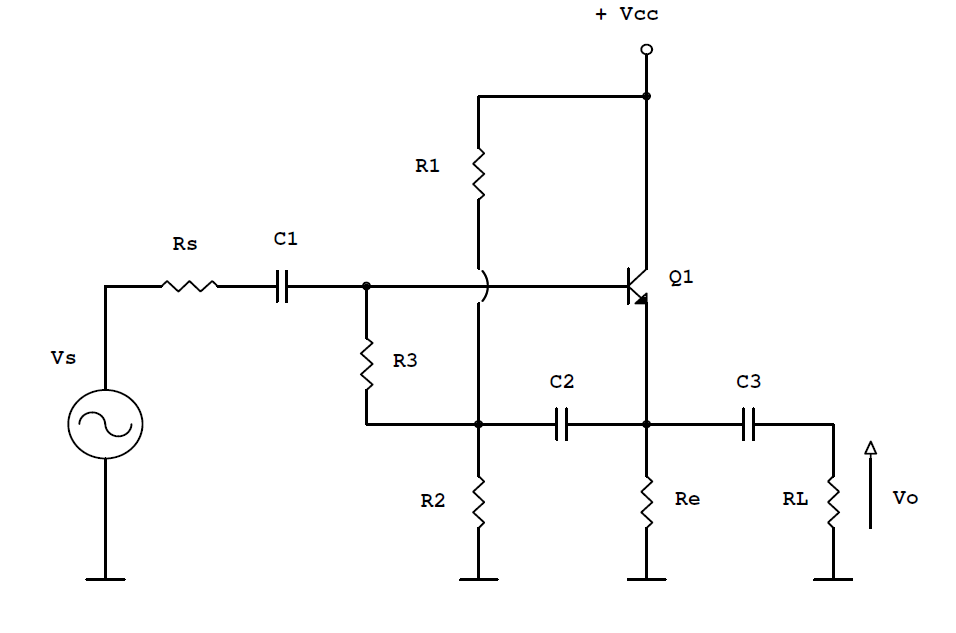
\includegraphics[width=0.8\textwidth]{imagenes/bootstrap.PNG}
	\caption{Circuito Bootstrap propuesto.}
	\label{fig:boot}
\end{figure}

\section{Desarrollo}

\subsection{Polarización}
El primer paso consiste en pasivar la fuente Vs y tratar los capacitores como un circuito abierto. Redibujando y utilizando el teorema de Thevenin se llega a las siguientes condiciones:
\begin{figure} [H]
	\centering
	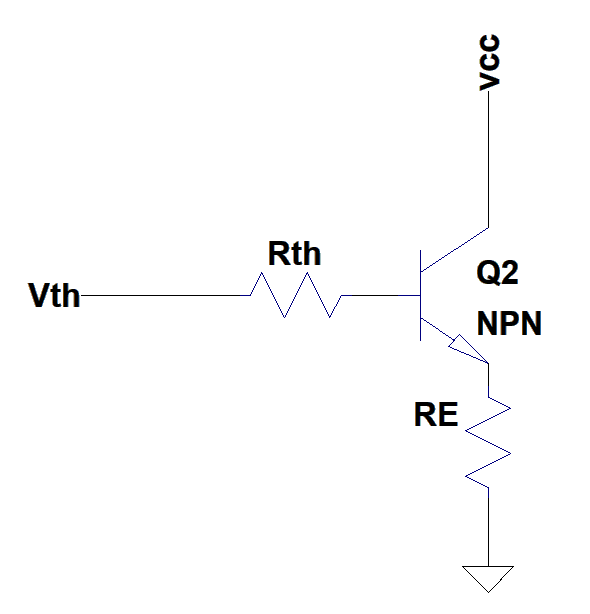
\includegraphics[width=0.5\textwidth]{imagenes/polarizacion.PNG}
	\caption{Circuito Bootstrap Polarización.}
	\label{fig:pol}
\end{figure}
donde:

\begin{equation*}
\left\{
\begin{aligned}
		& V_{Th}= V_{cc}\cdot \frac{R_2}{R_1+R_2} \\
		& R_{Th}= (R_1 // R_2) + R_3 
\end{aligned}
\right.
\end{equation*}

Recorriendo la malla de entrada se obtienen la siguientes ecuaciones:
\begin{equation*}
	V_{Th}-I_b \cdot R_{Th} -V_{BE_{On}}-I_e \cdot R_E=0  \ \  I_b\approx  \beta \cdot I_e
\end{equation*}

Es así que se consigue una expresión para $I_C$ con $V_{ce}$:
\begin{equation*}
	I_{C}\approx \frac{V_{Th}-V_{BE_{On}}}{\frac{R_{Th}}{1+\beta}+R_E} \ \ V_{ce} = V_{cc}-I_c\cdot R_E
\end{equation*}

\subsection{Modelo Incremental}
Para el modelo incremental se utilizarán los siguientes estimadores:
\begin{equation*}
\left\{
\begin{aligned}
	& \hat{hfe}=\beta \\
	& \hat{hie} = \frac{V_T}{I_b} \\
	& \hat{\frac{1}{hoe}} = \frac{V_a}{I_c}
\end{aligned}
\right.
\end{equation*}

Siendo este el circuito correspondiente al modelo:
\begin{figure} [H]
	\centering
	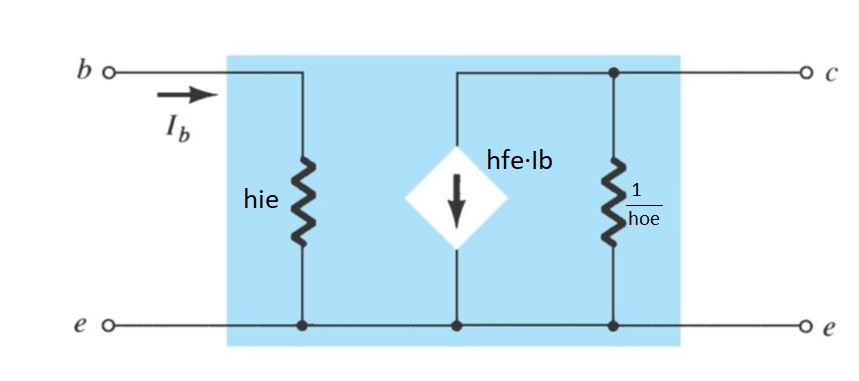
\includegraphics[width=\textwidth]{imagenes/modeloincremetnal.jpg}
	\caption{Modelo incremental.}
	\label{fig:modinc}
\end{figure}

Para el transistor utilizado en este infore, se midió HFE, siendo este $HFE \approx $
\begin{center}
	\textcolor{red}{\textbf{PONER HFE MEDIDO.}}
\end{center}

\subsection{Circuito Incremental}
Reemplazando el transistor por su modelo incremental, asumiendo que se trabaja con pequeñas señales a frecuencias medias, se obtiene el siguiente circuito:
\begin{figure} [H]
	\centering
	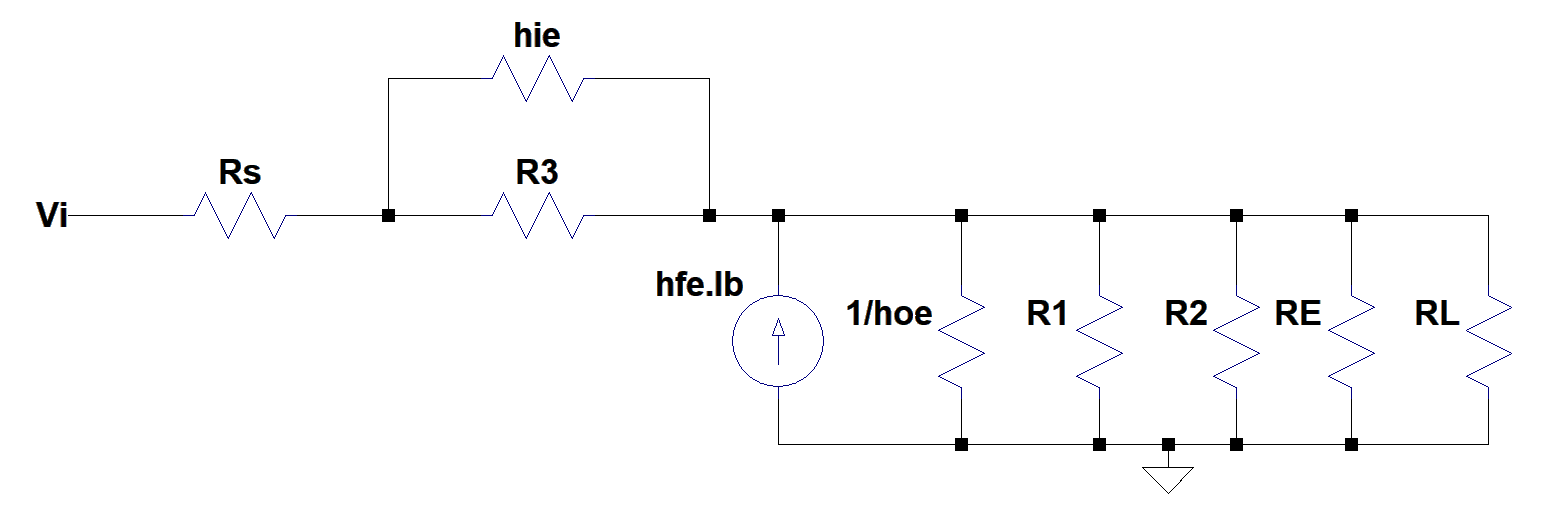
\includegraphics[width=\textwidth]{imagenes/circinc.png}
	\caption{Circuito incremental.}
	\label{fig:circinc}
\end{figure}

Redibujando convenientemente y utilizado el pasaje a nivel de corriente, se puede describir el circuito como:
\begin{figure} [H]
	\centering
	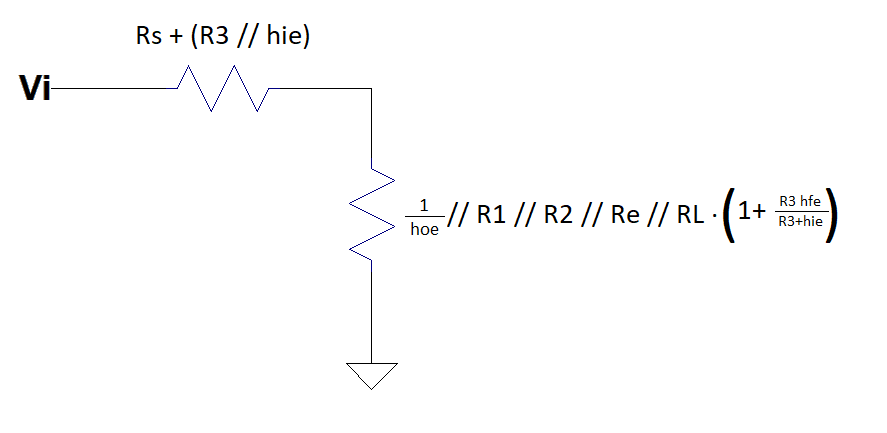
\includegraphics[width=\textwidth]{imagenes/circinc2.png}
	\caption{Circuito incremental final.}
	\label{fig:circinc2}
\end{figure}

Una pequeña modificacion que se hace a la expresión del circuito es definir un $hfe$ y un $hie$ efectivo. Para el circuito dado, estos son:
\begin{equation*}
\left\{
\begin{aligned}
	& hfe^* = hfe\cdot \frac{r_3}{R_3+hie} \\
	& hie^* = R_3 // hie
\end{aligned}
\right.
\end{equation*}

\subsection{Elección de componentes.}
Se eligió un punto de operación $Q$ tal que la tensión colector-emisor sea $V_{ce} = 5 \ V$, mientras que la corriente de colector sea $I_{cq} = 2 \ mA$. Se eligieron resistencia que cumplan dicho punto de polarización, recorriedo la malla de entrada y salida para determinarlos. Es así que se llegó a los siguientes valores: $R_1 = 10 \ k\Omega$, $R_2 = 14.7 \ k\Omega$, $R_3 = 1 \ k\Omega$ y $R_E = 2.2 \ k\Omega$.

Por otro lado, se tomó como resistencia del generador $R_s \approx 50 \ \Omega$, mientras que para la carga se consideró $R_L \approx 10 \ k\Omega$. Para los capacitores, sus valores nominales fueron elegidos tal que su impedancia sea despreciable frente a las resistencias frente a frecuencias medias.

\subsection{Resultados de interés.}
Se realiza un enfoque en la ganancia de tensión, corriente, impedancia de entrada y de salida:


\begin{equation}
	\Delta V \triangleq \frac{V_o}{V_i} = \frac{ \left(\frac{1}{hoe} // R_1 // R_2 // R_E // R_L  \right)\cdot (1+hfe^*)}{R_s + hie^* + \left(\frac{1}{hoe} // R_1 // R_2 // R_E // R_L  \right)\cdot (1+hfe*) } 
\end{equation}

\begin{equation}
	\Delta I \triangleq \frac{I_o}{I_i} =  
\end{equation}

\begin{center}
	\textcolor{red}{\textbf{COLOCAR GANANCIA DE CORRIENTE.}}
\end{center}

\begin{equation}
	Z_{In} = R_s + hie^* + \left(\frac{1}{hoe} // R_1 // R_2 // R_E // R_L  \right)\cdot (1+hfe*)
\end{equation}

\begin{equation}
	Z_{Out} = R_s + \left[ hie^* //  \left(\frac{1}{hoe} // R_1 // R_2 // R_E // R_L  \right) \right] \cdot (1+hfe*)
\end{equation}

\begin{center}
	\textcolor{red}{\textbf{VERIFICAR PRECEDENCIA.}}\\
	\textcolor{red}{\textbf{AGREGUÉ LOS CORCHETES Y CREO QUE ERA ASÍ.}}
\end{center}

Luego se graficó la ganancia de tensión en función de la frecuencia:
\begin{figure} [H]
	\centering
	\includegraphics[width=\textwidth]{imagenes/avs.png}
	\caption{Transferencia Módulo.}
	\label{fig:transmod}
\end{figure}
\begin{figure} [H]
	\centering
	\includegraphics[width=\textwidth]{imagenes/avsp.png}
	\caption{Transferencia Fase.}
	\label{fig:transph}
\end{figure}


\end{document}
